% Capítulo 4 – Proposta (Arquitetura e Design)
\chapter{Proposta de Arquitetura e Design}
\label{cap4}
\justifying

Este capítulo descreve a arquitetura técnica do artefacto \textbf{VotoChain} e detalha as decisões de design que atendem aos requisitos de integridade, anonimato verificável e transparência, bem como as diretrizes de usabilidade WCAG 2.1.

\section{Visão Geral da Arquitetura}
A solução está estruturada em três camadas principais (Figura~\ref{fig:arquitetura}):
\begin{enumerate}
    \item \textbf{Camada de Dados (Blockchain)} – rede pública Ethereum Sepolia onde residem os smart contracts responsáveis pelo registo de eleitores, submissão de votos e apuramento. Os Smart Contracts, conceito introduzido por Nick Szabo em 1997\cite{szabo1997formalizing}, são a base lógica do VotoChain. No nosso sistema, os contratos residem na \textbf{EVM} (Ethereum Virtual Machine) e são escritos em \textbf{Solidity}.
    \item \textbf{Camada de Anonimato} – módulo que dissocia a identidade do eleitor do voto usando \textbf{Zero-Knowledge Proofs (zk-SNARKs)} ou \textbf{Mix-Nets} (seleção feita após avaliação de custo/benefício).
    \item \textbf{Camada de Aplicação (Frontend)} – interface web desenvolvida em React + Ethers.js, projetada segundo WCAG 2.1 (nível AA) para garantir acessibilidade. O design universal, proposto por Mace (1997)\cite{universal_design}, foi adotado como princípio norteador. A camada de apresentação é o ponto de entrada para o eleitor. Desenvolvida em \textbf{React.js}, a interface foi projetada seguindo os princípios de acessibilidade \textbf{WCAG 2.1}\cite{accessibility_principles}.
\end{enumerate}

\begin{figure}[ht!]
\centering
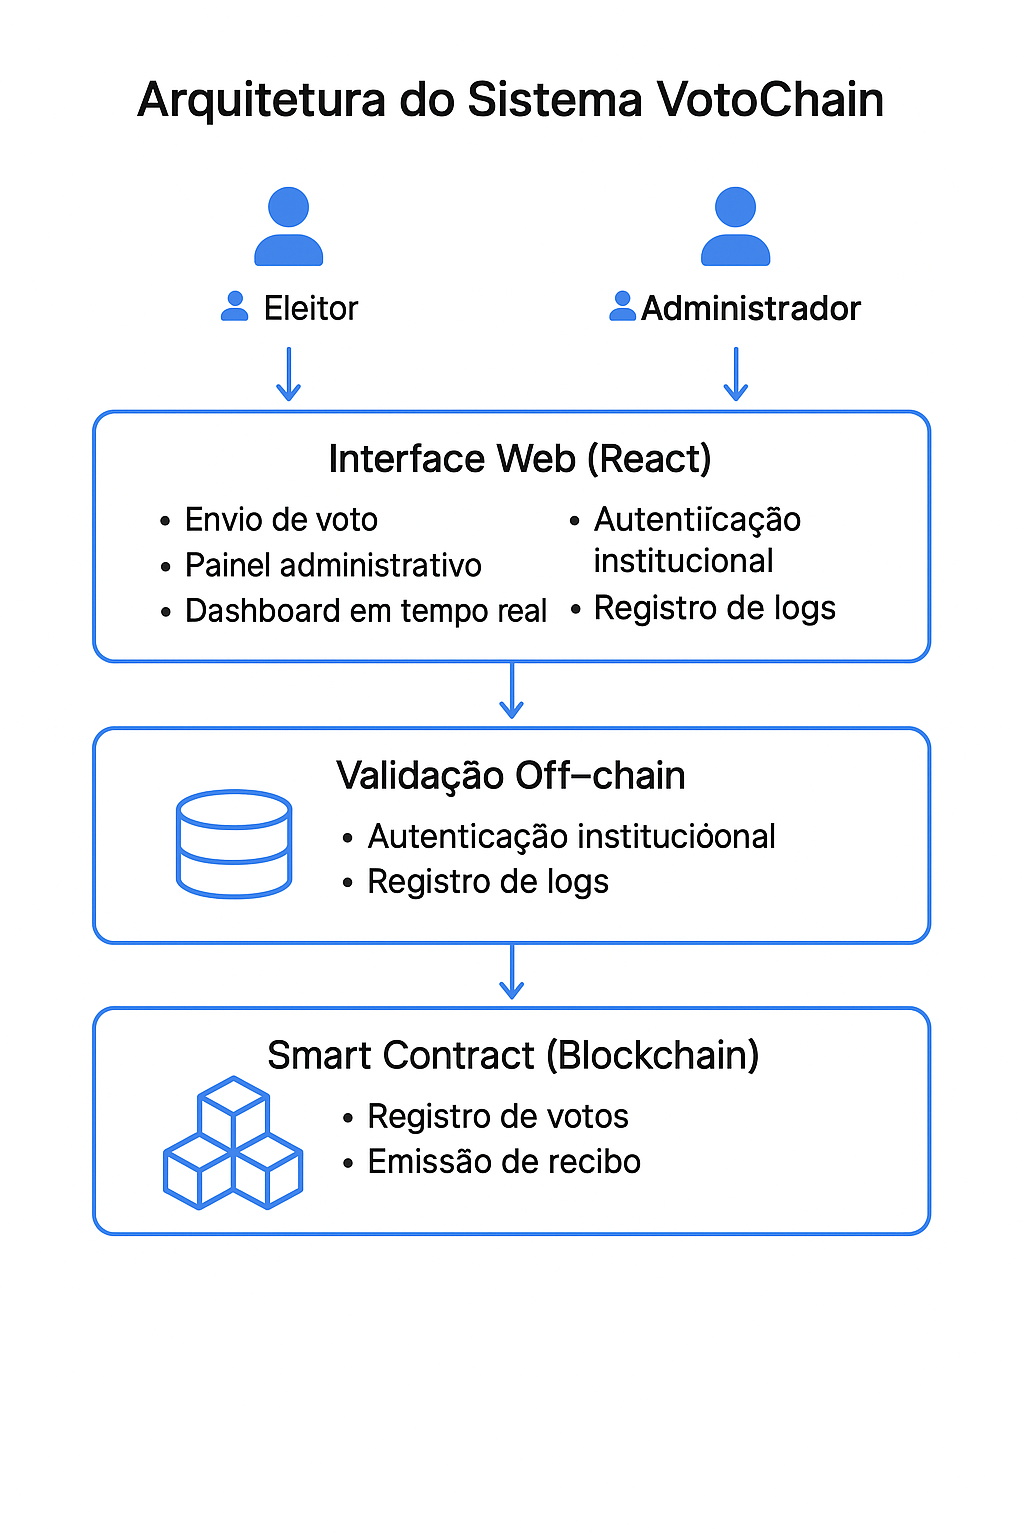
\includegraphics[width=0.8\textwidth]{figuras/Arquitectura_Sistema_VotoChain.png}
\caption{Arquitetura detalhada de três camadas do VotoChain: Frontend, Anonimato e Blockchain.}
\label{fig:arquitetura}
\end{figure}

\section{Componentes de Smart Contracts}
Os contratos são organizados em três módulos inter‑ligados:
\begin{enumerate}
    \item \textbf{RegistoEleitor.sol}\ – gere o cadastro de identidades digitais (endereço Ethereum ↔ identidade institucional). Utiliza um mapeamento `address => bytes32` e verifica a unicidade via `require(!registered[msg.sender])`.
    \item \textbf{VotoAnonimo.sol}\ – recebe o voto anonimizado (hash ou proof) e o armazena em uma estrutura `mapping(uint256 => bytes32) votes`. Cada voto recebe um identificador incremental e não pode ser alterado (`immutable`).
    \item \textbf{Apuracao.sol}\ – contabiliza os votos ao final da eleição, emitindo um evento `ResultPublished(uint256 totalYes, uint256 totalNo)`. O contrato inclui funções de *emergency stop* (`circuitBreaker`) para garantir a integridade em caso de ataque.
\end{enumerate}

Todos os contratos são compilados com Solidity \textasciicircum 0.8.20 e auditados com \textbf{Slither} e \textbf{MythX} para detectar vulnerabilidades de re-entrância, overflow e acesso não autorizado.

\section{Módulo de Anonimato}
Dois caminhos foram avaliados:
\begin{itemize}
    \item \textbf{ZK‑SNARKs}\ – gera‑se um proof off‑chain (via `snarkjs`) que comprova que o eleitor possui direito a votar sem revelar sua identidade. O proof tem tamanho ~200 bytes e consome ~150 000 units de gas por voto.
    \item \textbf{Mix‑Nets}\ – os votos são embaralhados entre três nós de mistura controlados por contratos de *relay*. Cada nó re‑encaminha o voto criptografado, removendo a associação direta ao endereço original. O custo médio é ~90 000 units de gas.
\end{itemize}
A escolha final será baseada nos resultados experimentais da Etapa 6 (Resultados), mas a arquitetura suporta a troca modular de ambos os mecanismos.

\section{Design da Interface (WCAG 2.1)}
A UI segue os princípios de design universal:
\begin{itemize}
    \item \textbf{Perceptível}: contraste mínimo 4.5:1, textos redimensionáveis, suporte a leitores de tela (ARIA labels).
    \item \textbf{Operável}: navegação completa via teclado, tempo de sessão ajustável, indicadores de foco visíveis.
    \item \textbf{Compreensível}: linguagem clara, instruções passo‑a‑passo, validação de formulários em tempo real.
    \item \textbf{Robusto}: código HTML5 semântico, componentes React testados com Jest + React Testing Library.
\end{itemize}

\section{Diagrama de Casos de Uso}
A Figura~\ref{fig:casos_uso} detalha as interações entre os atores (Eleitor e Administrador) e o sistema.

\begin{figure}[ht!]
\centering
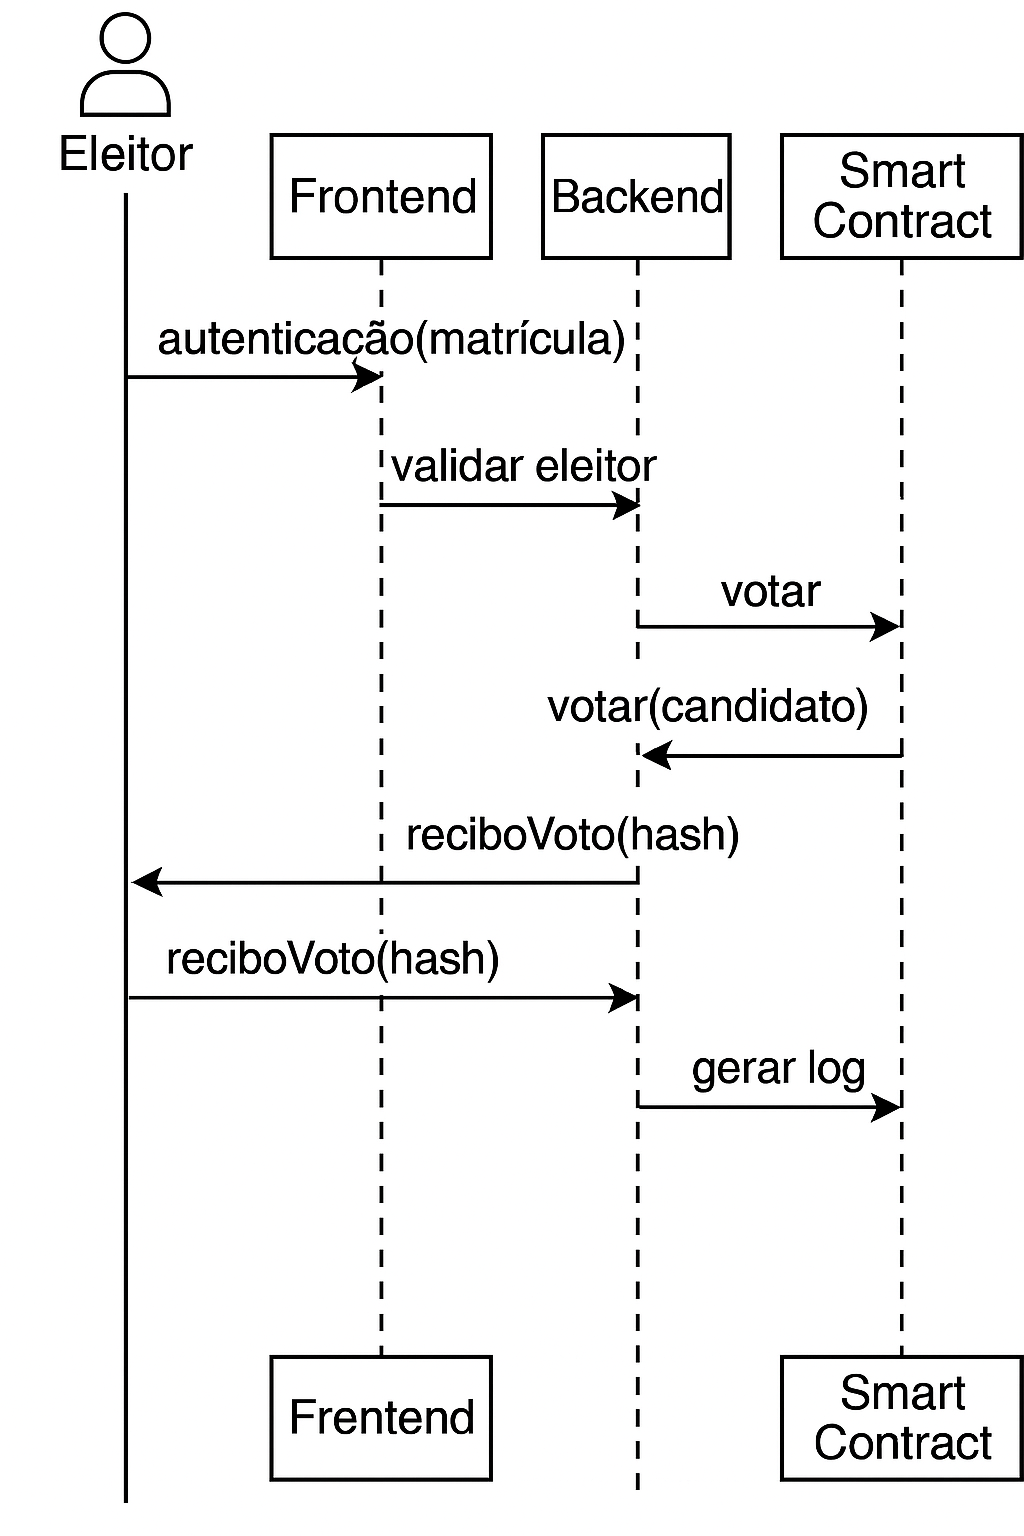
\includegraphics[width=0.7\textwidth]{figuras/Diagrama_Casos_de_Uso_VotoChain.png}
\caption{Diagrama de Casos de Uso do sistema VotoChain.}
\label{fig:casos_uso}
\end{figure}

\section{Fluxo de Votação – Diagrama de Sequência}
O fluxo detalhado de mensagens entre os componentes durante o ato de votar é apresentado na Figura~\ref{fig:sequencia}.

\begin{figure}[ht!]
\centering
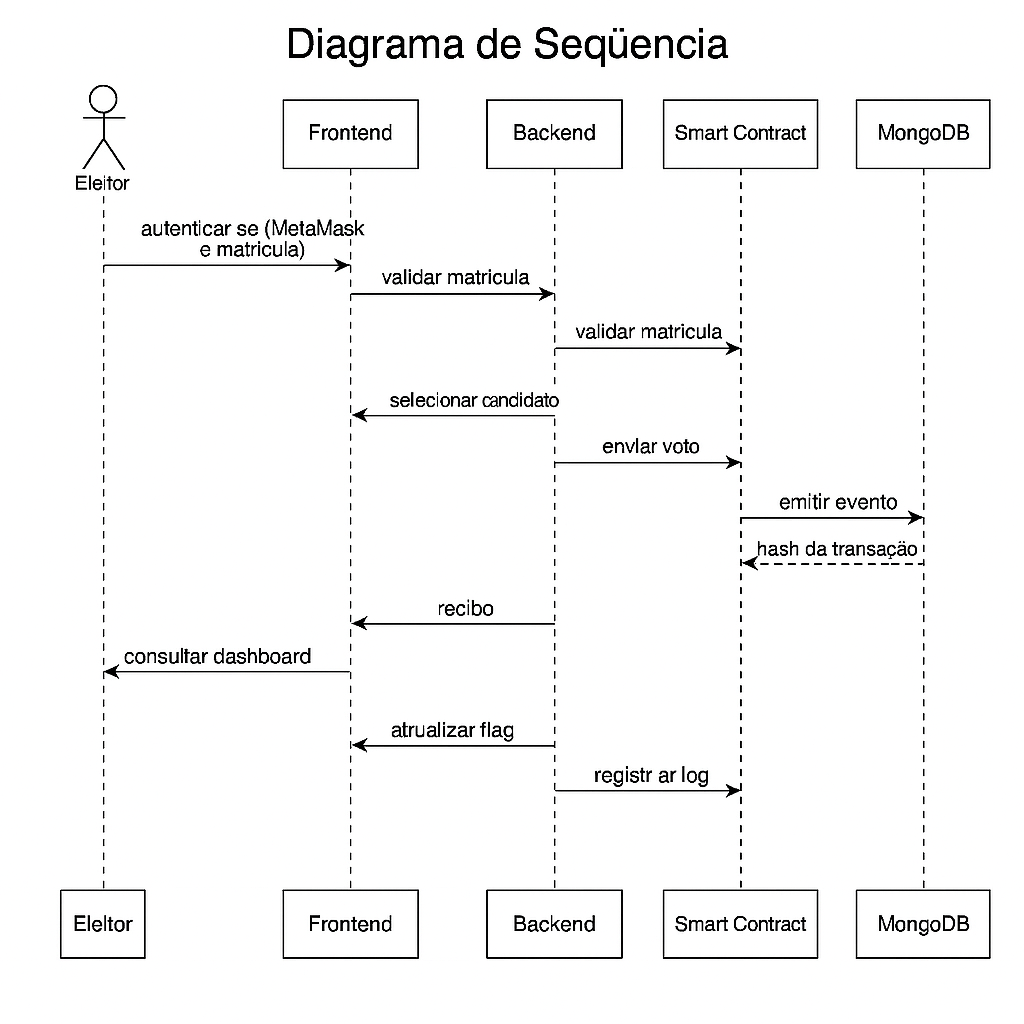
\includegraphics[width=0.9\textwidth]{figuras/Diagrama_Sequencia_VotoChain.png}
\caption{Diagrama de Sequência para submissão de voto anonimizado.}
\label{fig:sequencia}
\end{figure}

\section{Diagrama de Classes}
A estrutura de dados e as relações entre os Smart Contracts e módulos de suporte são ilustradas no diagrama de classes da Figura~\ref{fig:classes}.

\begin{figure}[ht!]
\centering
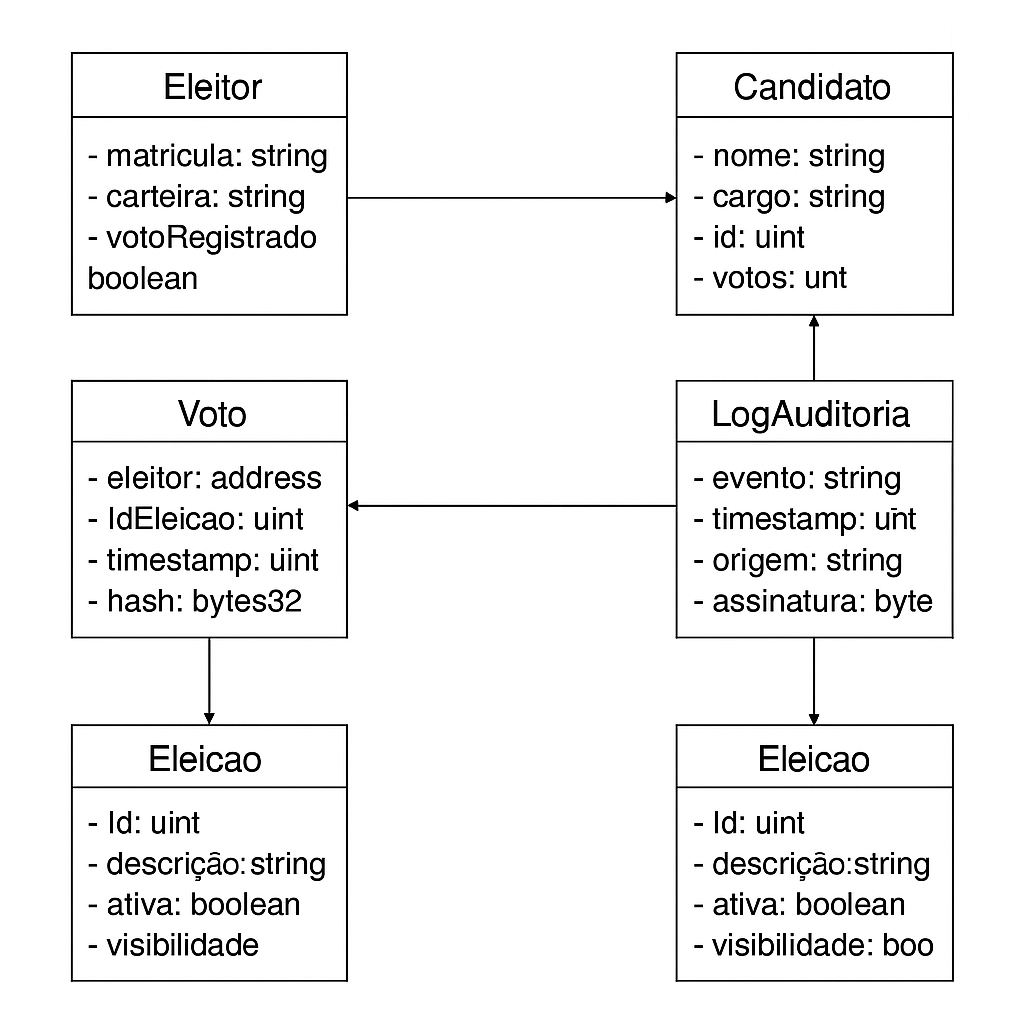
\includegraphics[width=0.9\textwidth]{figuras/Diagrama_Classes_VotoChain.png}
\caption{Diagrama de Classes dos Smart Contracts e Módulos do Sistema.}
\label{fig:classes}
\end{figure}

\section{Considerações de Segurança}
\begin{itemize}
    \item \textbf{Proteção contra replay}: cada proof inclui um nonce único armazenado no contrato.
    \item \textbf{Circuit Breaker}: o contrato `Apuracao.sol` pode ser pausado por um endereço de governança multi‑sig.
    \item \textbf{Auditoria externa}: o código será submetido a revisão por terceiros (e.g., ConsenSys Diligence) antes da publicação.
\end{itemize}

\section{Roadmap de Implementação}
\begin{enumerate}
    \item Implementar `RegistoEleitor.sol` e `VotoAnonimo.sol` com suporte a ZK‑SNARKs.
    \item Desenvolver protótipo de Mix‑Net e integrar ao contrato `VotoAnonimo.sol`.
    \item Construir UI React conforme WCAG 2.1 e conectar ao contrato via Ethers.js.
    \item Executar testes de carga (100‑200 eleitores) em Sepolia.
    \item Avaliar métricas (gas, latência, usabilidade) e decidir o mecanismo de anonimato final.
    \item Documentar e publicar o código‑fonte.
\end{enumerate}


